\section{Automação}
\label{sec:auto}

Automação consiste na execução automatica de um processo com o mínimo de
intervensão humana. Para a área de TI, a automação ocorre nos processos de
controle e administração de sistemas ou softwares~\cite{sharma:2015}.

Pode-se citar algumas das vantagens da automação~\cite{sharma:2015}:
\begin{itemize}
  \item Ajuda a reduzir a complexidade de um processo;
  \item Ajuda a reduzir possibilidade de erros humanos em tarefas
    repetitivas;
\end{itemize}

\citeonline{sharma:2015} aborda as necessidade de se adotar automação na área
de TI (Tecnologia da Informação) e relaciona com os conceitos como métodos
ágeis, entrega contínua, computação em nuvem, etc. Além disso, são citados
os benefícios da automação mapeados com as principais preocupações da industria
de TI. Algumas delas:
\begin{itemize}
  \item \textbf{Agilidade}: promove pontualizada de agilidade para a TI. Em conjunto
    com os métodos ágeis resulta em múltiplas implantações em um curto intervalo
    de tempo;
  \item \textbf{Escalabilidade}: a automação ajuda a transformar a infra-estrutura
    em códigos simples, ou seja, a construção, reconstrução e configuração é possível
    ser feita em poucos minutos;
    \item \textbf{Precisão de Implantação}: 
\end{itemize}

\subsection{Infraestrutura como Código}

\subsection{Chef}
\label{sec:chef}

Chef é uma ferramenta de gerenciamento e configuração de infraestrutura criada
pela comunidade Opscode em 2008 oficialmente lançada em 2009. Seu propósito é
auxiliar na transformação de uma complexa infraestrutura em código, com nível
de abstração compreensiveis para os desenvolvedores. Sendo assim,
a gerência de configuração gira em torno da codificação simplificada e amigável
ao invés de comandos manuais de instalação e configuração de aplicações
\cite{sharma:2015}.

\begin{figure}[h]
  \label{fig:arch_chef}
  \centering
  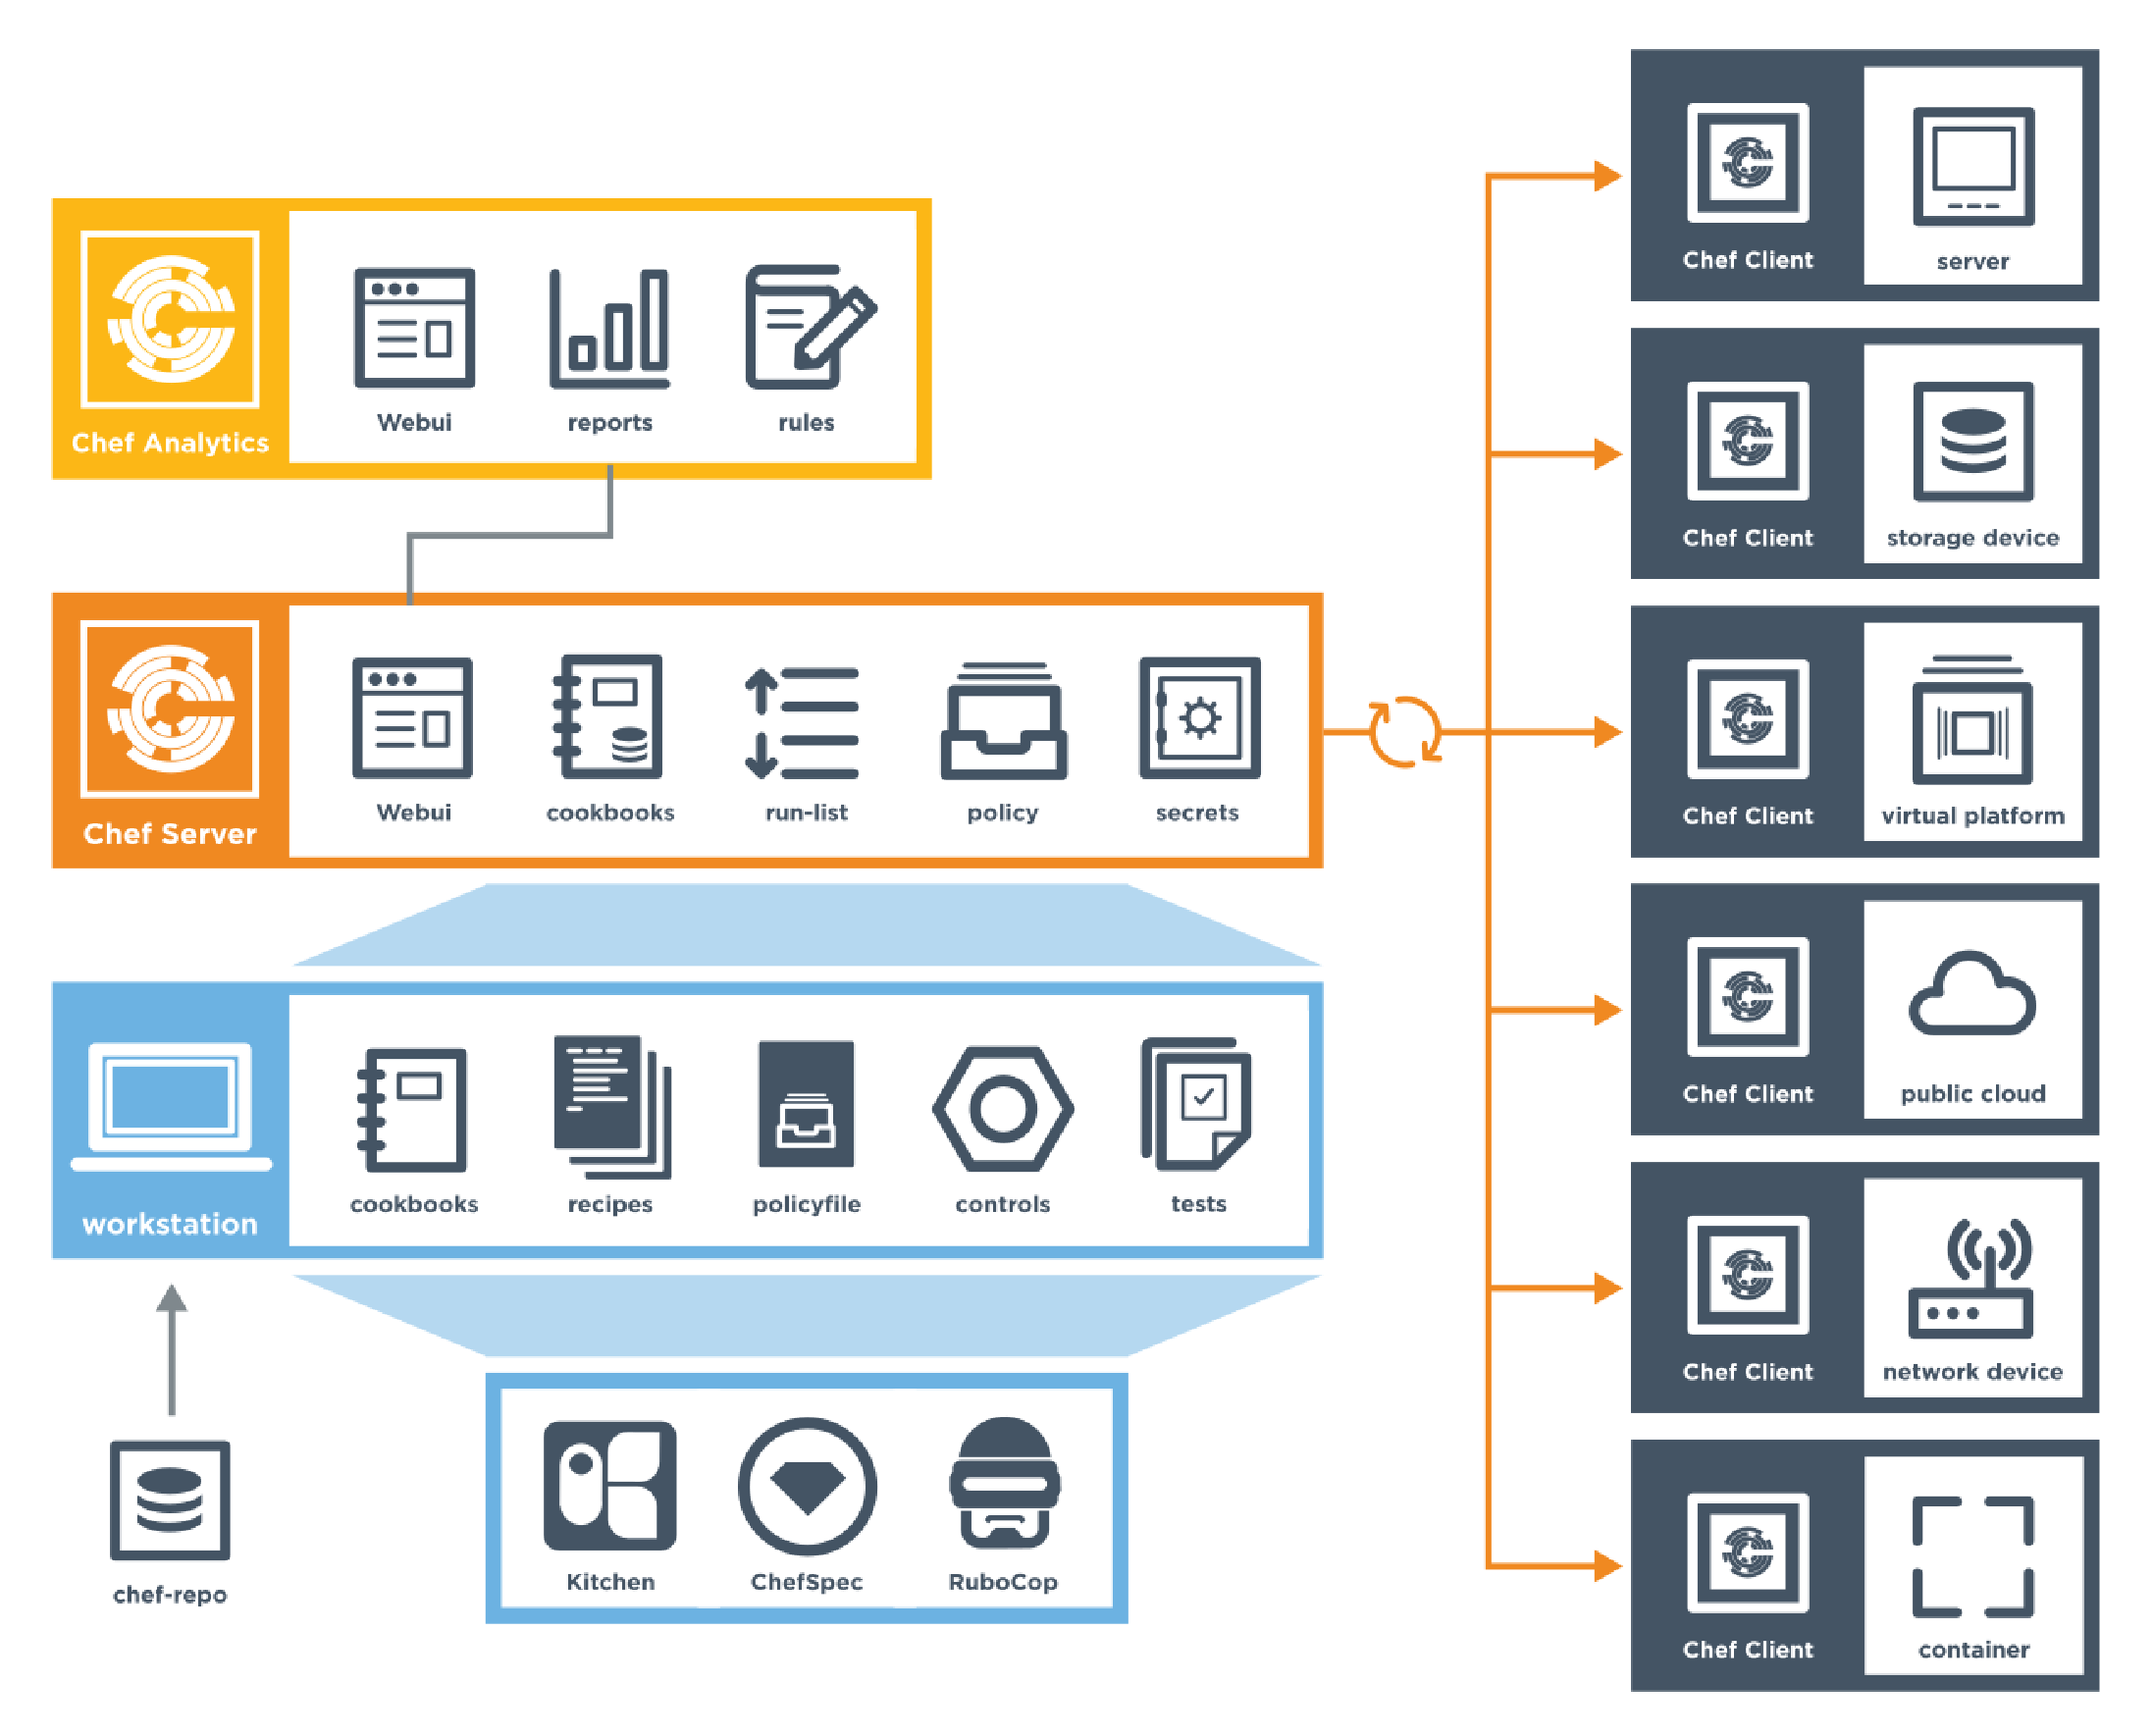
\includegraphics[width=\textwidth]{figuras/arch_chef.eps}
  \caption{Chef - Arquitetura de Componentes}
\end{figure}


